\documentclass[bachelor,winfonts]{jnuthesis}
\usepackage{listings}
\usepackage{float}

% 论文标题
\titlea{人工智能应用——聊天机器人的}
\titleb{开发}

% 论文作者姓名
\author{谭啸}
% 论文作者学生证号
\studentnum{1030413620}
% 导师姓名职称
\supervisor{徐华}
\supervisorpos{副教授}
% 第二行导师姓名职称,仿照第一行填写,没有则留空
\supervisorb{}
\supervisorbpos{}
% 论文作者的学科与专业方向
\major{计算机科学与技术}
% 论文作者所在院系的中文名称,学士学位论文此处不带“学院”二字
\department{物联网}
% 论文作者所在学校或机构的名称。此属性可选,默认值为``江南大学''。
\institute{江南大学}
% 学士学位获得日期,需设置年、月,默认为编译日期。
%\bachelordegreeyear{2017}
%\bachelordegreemonth{6}

\begin{document}
\lstset{
%% numbers=left, 感觉行号太丑了
%% numberstyle=\normalsize\itshape,
%% numbersep=5pt,
frame=lines,
%% escapeinside={\`}, 看起来已经支持中文了。
xleftmargin=2em,
xrightmargin=2em,
aboveskip=1em,
breaklines=true,
postbreak=\raisebox{0ex}[0ex][0ex]{\ensuremath{\color{red}\hookrightarrow\space}},
basicstyle=\normalsize\ttfamily,
}


% 制作中文封面
\maketitle

% 开始前言部分
\frontmatter

% 论文的中文摘要
\begin{abstract}
一、设计任务来源。聊天机器人是目前社会的热点,许多服务商在软件中集成了聊天机器人,来取代部分人工咨询的任务。聊天机器人在我们生活中的应用已经非常广泛了。各大公司都纷纷推出了自家的聊天机器人。但是,聊天机器人在如今也不是只有大公司可以提供的特权服务,因为依靠一种新兴的服务——聊天机器人平台,就可以让个人用户或小公司,定制属于自己的聊天机器人,同时只需要比较低的服务购买支出。Facebook Messenger 是最早的且流行最快的平台之一,10 亿多每个月活跃用户。在 Facebook 向外界尤其是开发人员开放了他们的机器人平台,在短短几个月内,就已有 23,000 多名程序开发者开始构建机器人并投入生产环境了。另外今年有一个以提供公司团队群组消息发布平台服务的公司,渐渐成为了人们讨论的热点。截至 2016 年 2 月,它每月拥有 230 万活跃用户,而且这一数字依然在快速增长。Slack 是当前的聊天机器人复兴浪潮中的先驱之一。为了小公司和个人用户也能拥有自己的聊天机器人,国外的许多公司推出了聊天机器人平台的服务,通过这些服务,用户只需要学习一定的使用规则,就能创建自己的聊天机器人了。但是他们有的依然是基于传统的 AIML 系统构建的,用户不得不学习晦涩且难于记忆的 AIML 标签。同时,国内基于 AIML 的聊天机器人平台很少,有部分原因是因为 AIML 不对英语国家之外的国家提供官方支持。

二、设计标准。本文以试图解决上述问题作为切入点,剖析了 AIML 源码和学习作者发表的文章,提出了开发聊天机器人的新的方案。

首先,确定了实现的功能和 ALICE 保持基本一致,但只实现其中一个子集。然后,摒弃全部的 AIML 模板规则,并设计新的规则。采用 Python3 开发,模板编码都采用 UTF-8,自然解决了 ALICE 对中文的不支持的问题。最后,使用 Web App 的形式,采取 MVC 结构,基于 AngularJS 开发了聊天机器人的界面,界面上具备的功能有基础的聊天功能,输入框,显示窗;注册登录页面;训练按钮。

三、设计原则。采取了需求驱动开发。由于本项目重点是聊天机器人的实现,主要工作在于思考一个优雅的设计方案,怎么降低模板编写的复杂度和冗余,因此不会放太多精力在它的界面上。所以,采取前后端分离,并且优先实现聊天机器人部分的功能,前端的功能只是提供一个 demo 的作用。另外,开发过程中还需要编写完善的单元测试,来保证程序的正确性。系统全部部署在了线上,开放给了用户使用,运行效果要一直保持良好。

四、主要技术资料。AIML 和 ALICE 官网;Github 里的源代码和网上的博客;已有的学术论文。


\keywords{聊天机器人;AIML;中文分词;JSON}
\end{abstract}

% 论文的英文摘要
\begin{englishabstract}
1. The design task source. Chat robot is the current social hot spots, many service providers in their software integrated chat robot, to replace some of the task of manual advice. Chat robots's application in our lives has been very wide. The major companies have launched their own chat robot. However, only a large company can provide the privilege service of chat robots, because relying on a new service - chat robot platform, you can let individual users or small companies, customize their own chat robots, and only need to compare Low service purchase expenses. Facebook Messenger is one of the earliest and most popular platforms, more than 1 billion active users per month. In the past few months, more than 23,000 programmers have started building robots and putting into production environments, where Facebook has opened up their robot platforms to the outside world, especially developers. In addition, this year there is a company to provide company team news release platform services company, has gradually become a hot discussion. As of February 2016, it has 2.3 million active users per month, and this figure is still growing rapidly. Slack is one of the pioneers of the current chat robot revival. For small companies and individual users can have their own chat robots, many foreign companies launched a chat robot platform services, through these services, users only need to learn a certain use of the rules, you can create your own chat robot. But some of them are still based on the traditional AIML system to build, the user had to learn obscure and difficult to remember the AIML label. At the same time, there are few platforms for domestic AIML-based chat robots, partly because AIML does not provide official support to countries outside of English-speaking countries.

2. the design standards. In this paper, we try to solve the above problems as a starting point, analyze the AIML source code and study the author's article, and propose a new scheme for developing chat robots.

First, it is determined that the implemented functionality is consistent with ALICE, but only one of the subsets is implemented. Then, abandon all the AIML template rules and design new rules. Using Python3 development, the template code are used UTF-8, ALICE naturally solve the problem of Chinese support. Finally, the use of Web App form, take the MVC structure, based on AngularJS developed a chat robot interface, the interface has the function of the basic chat function, input box, display window; registration login page; training button.

3. the design principles. Took a demand-driven development. As the focus of this project is to achieve the chat robot, the main work is to think about an elegant design, how to reduce the complexity of writing templates and redundancy, so will not put too much energy in its interface. So, to take the front and rear separation, and give priority to the function of the chat robot part, front-end function is to provide a demo role. In addition, the development process also need to prepare a perfect unit test, to ensure the correctness of the program. The system all deployed in the online, open to the user to use, the operation effect should always be good.

4. the main technical information. AIML and ALICE official website; Github source code and online blog; existing academic papers.

% 英文关键词。关键词之间用英文半角逗号隔开,末尾无符号。
\englishkeywords{Chatbot, AIML, Chinese word segmentation, JSON}
\end{englishabstract}

% 生成论文目录
\tableofcontents

% 开始正文部分
% 大概 30 行,为 1 页。
\mainmatter

\chapter{绪论}\label{chapter_introduction}
\section{聊天机器人的定义及背景}
聊天机器人是什么?聊天机器人是一种通过自然语言模拟人类进行对话的程序。通常运行在特定的软件平台上,如PC平台或者移动终端设备平台,而类人的硬件机械体则不是必需的承载设备。

聊天机器人的研究源于图灵(Alan M. Turing)在1950年《Mind》上发表的文章《Computing Machinery and Intelligence》,文章开篇提出了“机器能思考吗?”的设问,并且通过让机器参与一个模仿游戏来验证“机器”能否“思考”,进而提出了经典的图灵测试。图灵测试被认为是人工智能的终极目标,图灵本人因此也被称作“人工智能之父”。

“聊天机器人”(ChatterBot)这个术语最早由麦可·洛伦·莫尔丁(Michael Loren Mauldin,开发了第一个Verbot,Julia)于1994年时在谈话节目中提及。最早的聊天机器人 ELIZA 诞生于1966年,由麻省理工学院(MIT)的约瑟夫·魏泽鲍姆(Joseph Weizenbaum)开发,用于在临床治疗中模仿心理医生。值得注意的是尽管ELIZA的实现技术仅为关键词匹配及人工编写的回复规则,但魏泽鲍姆本人对ELIZA的表现感到吃惊,随后撰写了《Computer Power and Human Reason》这本书,表达他对人工智能的特殊情感。

为了进一步将图灵测试付诸实践,美国科学家兼慈善家休·勒布纳(Hugh G. Loebner)于1990年设立了人工智能年度比赛——勒布纳奖(Loebner Prize)(包括10万美金的奖金和一块印有勒布纳与图灵头像的金牌)。勒布纳奖的设立旨在奖励首个与人类回复无差别的计算机程序,即聊天机器人系统,并以此推动图灵测试及人工智能的发展。在勒布纳奖的推动下,聊天机器人的研究迎来了一个高潮,这里面较为代表性的聊天机器人系统是ALICE(Artificial Linguistic Internet Computer Entity)\cite{alicewebsite}。受到ELIZA聊天机器人的启发,理查德·华勒斯(Richard S. Wallace)博士在1995年开发了ALICE系统。ALICE曾经在2000年、2001年和2004年三次问鼎勒布纳奖,并于1998年开始开源,目前全世界有超过500个开发者为ALICE项目贡献代码。值得注意的是,随着ALICE一同发布的AIML(Artificial Intelligence Markup Language)目前被广泛应用在移动端虚拟助手的开发中。尽管ALICE采用的是启发式模板匹配的对话策略,但是它仍然被认为是同类型聊天机器人中性能最好的系统之一。而本文研究的内容,也与 ALICE 系统密切相关。


\section{国内外研究现状}
从1995年开始,互联网得到快速发展,各式各样的聊天机器人系统也不断出现在公众视线里。各个公司巨头几乎都着手或已实现自己的机器人。

从技术层面来看,从上一节我们初步得知聊天机器人一开始是基于规则匹配的,即预先将回答存储,然后提取问句中的关键词和主题,通过一定的算法,来查找预先存储好的回答数据库,构建这样的聊天机器人相对简单,目前市面上有很多公司依然是基于类似的算法实现自家聊天机器人的,虽然简单,可效果并不差。

目前深度学习也是另一个极热的热点,基于神经网络的对话模型\cite{seq2seq},打开了聊天机器人开发的另一片天地。这种方式,不再需要检索数据库,而是将输入翻译为输出(图\ref{fig:pic1}),能够自己生成句子。Google 开源了 tensorflow 深度学习框架,可以让普通开发者在本地搭建一个运行深度学习的环境。

\begin{figure}[htbp]
  \centering
  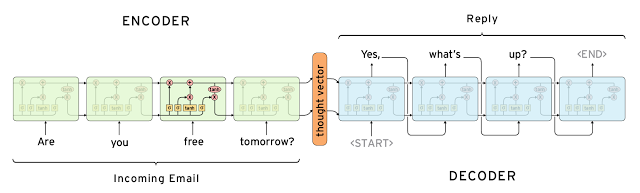
\includegraphics[width= 1\textwidth]{nct-seq2seq.png}\\
  \caption{输入翻译到输出}\label{fig:pic1}
\end{figure}

从应用场景分类来看,比较活跃的有在线客服、公共聊天、个人助理等种类\cite{chinaAI}。在线客服聊天机器人的主要功能是与用户进行基础的沟通,回复用户对公司的产品或者服务的咨询,这样能有效的降低客服的运营成本。应用场景通常为大厅立式终端,或者微信公众号。代表性的系统有京东的JIMI客服机器,银行的咨询和取号机器人等。用户可以通过与JIMI聊天了解商品的详细信息,价格,以及反馈购物中存在的问题等。值得称赞的是,JIMI具备一定的拒识能力,能够知道自己不能回答用户的哪些问题,准确的将此次会话转向人工客服。公共聊天室场景的聊天机器人,能根据聊天主题的改变,以及进入聊天室的用户等因素,做出反应。国外的某些商业网站就有一些有趣的聊天机器人,比如 github 推出的 HUBOT,它更像是一个可配置脚本机器人,能够在特地的聊天室环境,自动完成很多工作,目前已经开源。个人助理类应用主要通过,语音或文字与聊天机器人系统进行交互,实现个人事务的查询及代办功能,如天气查询、空气质量查询、旅游住宿查询、电影片购买、酒店预订、餐饮等,对用户的生活质量带来了很大提升。一般这类机器人都是以 App 的形式使用的,代表性的 App  有百度的小度、新浪微博机器人、Apple的Siri、Google的Now、微软小娜等。Apple的Siri更是为广大果粉津津乐道。Apple的Siri本体集成在 iOS 系统中,用户可以简单的摁下 home 键唤起,支持的交流方式有点触、语音。在 Siri 刚开始发布的时候,受聊天机器人业整体发展水平限制,并没有带来太大的关注,但随着 iOS 系统的迭代和科技的进步,Siri 已经变得非常实用了。

然而,聊天机器人并不是大公司才有的“专利”,一种新兴的服务——聊天机器人平台,让个人用户或小公司,能够以比较低的成本,定制属于自己的聊天机器人。Facebook Messenger 是最流行的消息平台之一,每月拥有 10 亿多活跃用户。在 Facebook 向开发人员开放其机器人平台几个月内,已有 23,000 多名开发人员在构建机器人。目前为止,他们已发布了 18,000 多个机器人。Facebook Messenger 机器人与 Facebook 页面紧密相关,这在企业中非常普遍。Slack 是一个适合工作相关团队的群组消息平台。截至 2016 年 2 月,它每月拥有 230 万活跃用户,而且这一数字正在快速增长。Slack 是当前的聊天机器人复兴浪潮中的先驱之一。Slack 提供了业界第一个 “机器人商店”,使团队能更轻松地发现和安装机器人。不出所料,大部分 Slack 机器人都与工作和生产力有关。国内的微信,每月活跃用户有7亿多,企业通常在建立网站很久以前就已经拥有了微信机器人。


\section{存在的主要问题}
从宏观上来说,目前聊天机器人的实现,依然存在一些公认的难题和挑战。其中包括:如何利用好上下文信息,如何解决通用回复问题以及如何计算一次会话的好坏与质量。

一个好的聊天机器人应该能够结合上下文进行回复。在长对话中,人类可以跟踪说过的人名,地名,心情信息等等。如何有效利用长对话中的信息成为研究的热点问题。聊天机器人中另一个常见的问题是,在基于生成的方法中倾向于生成通用的回复,像“很好”,“我不知道”,这些在大多情况下适用的回复。针对这种问题,很多研究者试图通过改变目标函数来提高回复多样化。如何评价一个模型结果的好坏同样是聊天机器人实现的一个难点。由于在回复中可能会包含完全不同的单词或者短语,因此机器翻译中常用的评估矩阵 ELEU 并不适合用来作为聊天机器人的评价矩阵。

从国内的广泛应用来说,已有的聊天机器人的实现比如 AIML ,基于一些历史原因,API实现并不完美,导致模板规则的编写难度较大,而且 AIML 内置的分词手段是基于空格来分隔英文单词的,而中文没有单词一说,所以必须依赖外部分词工具,因此想使用 AIML 必须改写内部一些代码。

\section{论文主要研究内容}
本文主要工作是剖析 AIML 核心,并实现一个新的版本(Json Robot)。针对目前网络上越来越多的聊天机器人平台的发布,他们有些是基于 AIML 设计的,既需要每个用户都学习晦涩的 AIML 语法,因此设计一个模板书写简洁易懂,并且可配置插件的机器人是一件很有意义的事情。

新版本必须具备 AIML 的基本功能,同时拥有一些创新点,具体对比请看(表\ref{table:t1})。

\begin{table}[ht!]
  \centering
  \begin{tabular}{cp{38mm}p{38mm}}
    \toprule
    \textbf{} & \textbf{Json Robot} & \textbf{AIML}\\
    \midrule
    模板编写  & json文件,key-value的形式,语义化编写 &  xml文件,树状形式,需要阅读大量说明才能编写   \\
    \hline
    支持的功能     & 
    \begin{enumerate}
    \item 基本的匹配规则
    \item 答案随机返回
    \item 重定向搜索
    \item 问与答之间的关系是多对多
    \item 可配置插入第三方模板
    \end{enumerate} &
    \begin{enumerate}
    \item 基本的匹配规则
    \item 答案随机返回
    \item 重定向搜索
    \item 问与答之间的关系是多对多
    \item 基于存储对话关键信息的方式关联上下文
    \end{enumerate} \\
    % \\1.重定向搜索\newline2.答案随机返回\newline3.基本的匹配规则\newline4.问与答之间的关系是多对多\newline5.可配置插入第三方模板  &  1.重定向搜索\newline2.答案随机返回\newline3.基本的匹配规则\newline4.问与答之间的关系是多对多\newline5.基于存储对话关键信息的方式关联上下文   \\
    \hline
    存储形式     & 本地磁盘 + 索引文件    &  通常基于数据库   \\
    \hline
    读取方式及速度     & 通过文件路径打开文件,快     & 连接并查询数据库,慢 \\
    \hline
    内部设计    & 现代API的设计,模块化   &  复杂(可以参考已有的Python实现,同样的功能 Json Robot 所需代码更少)   \\
    外部接口    & 简单   &  简单\\
    \bottomrule
  \end{tabular}
  \caption{AIML和Json Robot对比}\label{table:t1}
\end{table}

本文一共分为五章。

第一章简要介绍了聊天机器人的历史和发展状况,以及面临的挑战。

第二章主要介绍了 AIML 的核心匹配算法。AIML 是一个开源机器人,关于它的匹配规则,这篇文章有详细介绍\cite{aiml-match-pattern}。这是程序的核心所在,所有的其他的搜索逻辑都将成为这部分的扩展。

第三章介绍了中文分词。本项目采用的是 Bosonnlp 公司的分词技术,采取调用第三方 Restful API 的形式。该服务能提供的功能其实并不仅仅只有分词,还有关键词提取,情感分析等,这些都是聊天机器人可以利用的增强工具。

第四章介绍了本系统(Json Robot)的详细设计过程。包括系统的前后端架构,编码的模块化,良好的测试保障,以及用户界面的设计等。

第五章是总结。一方面总结了项目的最终实现效果,另一方面对需要增强的地方也提出展望。聊天机器人的热度依旧会持续下去。


\chapter{ALICE和AIML}
\section{ALICE的工作原理及其优缺点}
\subsection{ALICE的工作原理}
ALICE \cite{夏天2004基于}是人工语言在线机器人(The Artificial Linguistic Internet Computer Entity)的缩写,是一个可以聊天的程序。 ALICE 的知识库是存在 AIML 文件中的,AIML 是人工智能标记语言的缩写(The Artificial Intelligent Mark up Language),它相当于可扩展标记语言 XML 的一种派生。

剖析 ALICE 的工作原理,可以从源代码出发。因为 ALICE 有很多语言的实现,而本项目是 python 实现的,所以就来看同样是 python 实现\cite{github-pyaiml}的 ALICE。

\begin{figure}[htbp]
  \centering
  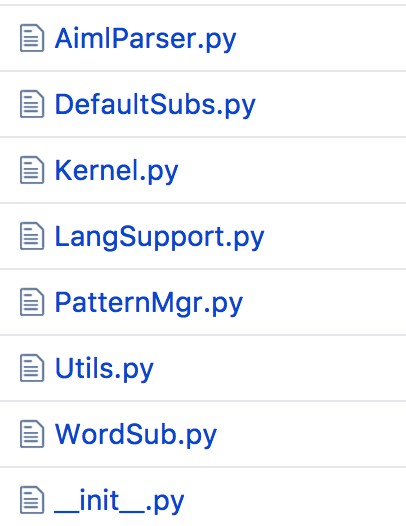
\includegraphics[width= 0.35\textwidth, height=0.45\textwidth]{pyaiml-project.png}
  \caption{pyaiml 源代码}\label{fig:pic2}
\end{figure}


我们根据数据的流向来跟踪程序运行。首先,我们有一个人工编写的AIML文件。

\begin{lstlisting}[language=XML]
<aiml version="1.0">
<category>
<pattern>* 再见</pattern>
<template>
谢谢你陪我聊天
</template>
</category>
</aiml>
\end{lstlisting}

这个例子很简单,<category> 标签代表一个基本的对话单元,<pattern> 标签里的内容对应对话里的问句,其中的通配符,比如例子里的 * 代表的含义会在后面解释。然后 <template> 标签里的内容对应对话里的回答。接下来看文件是怎么被读入的。

\begin{lstlisting}[language=Python]
 def learn(self, filename):
        for f in glob.glob(filename):
            # Load and parse the AIML file.
            parser = AimlParser.create_parser()
            handler = parser.getContentHandler()
            handler.setEncoding(self._textEncoding)
            try: parser.parse(f)
            except xml.sax.SAXParseException, msg:
                err = "\nFATAL PARSE ERROR in file %s:\n%s\n" % (f,msg)
                sys.stderr.write(err)
                continue
            # store the pattern/template pairs in the PatternMgr.
            for key,tem in handler.categories.items():
                self._brain.add(key,tem)
\end{lstlisting}

在 Kernel.py 里可以看到,程序根据文件名(带通配符)读入多个文件,将文件名传给了 parser 实例,parser成功后返回的结果为 pattern/template 的字典,被存到了 PatternMgr 里(之后会介绍)。我们之前已经知道了 AIML 文件里有很多标签,而 ALICE 之所以能支持这么丰富的功能,秘密全在这些标签里面,现在来看 AIML 具体是如何被解析的。

\begin{lstlisting}[language=Python]
from xml.sax.handler import ContentHandler
...
class AimlHandler(ContentHandler):
...
_validationInfo101 = {
    ...
    "system":       ( [], [], True ),
    "template":		  ( [], [], True ),
    "that":         ( [], ["index"], False ),
    "thatstar":     ( [], ["index"], False ),
    "think":        ( [], [], True ),
    "topicstar":    ( [], ["index"], False ),
    "uppercase":    ( [], [], True ),
    "version":      ( [], [], False ),
}
...
\end{lstlisting}


如上所示,在 AimlParser.py 中,我们可以看到程序利用了 python 的 xml 库来处理。继承并覆盖了原来的handler,这样 AIML 文件被读入后会被验证编写是否符合规范,不符合规范的文件会报错,并且指出错误的位置。


\begin{lstlisting}[language=Python]
    ...
    def _respond(self, input, sessionID):
        # Determine the final response.
        response = ""
        elem = self._brain.match(subbedInput, subbedThat, subbedTopic)
        # Process the element into a response string.
        response += self._processElement(elem, sessionID).strip()
        return response
\end{lstlisting}

如上所示,在 Kernel.py 里面,输入的问句首先会经过匹配机制,也就是传统意义上所说的搜索数据库的过程,这里的数据可以看做都存在了内存里。返回的结果是一颗含有回答模板的元素树,这颗元素树之后会被一系列函数分析并产生最终的字符串表示的结果,返回给用户。

下面重点介绍这个匹配机制\cite{aiml-match-pattern}。该匹配机制是由 Richard S. Wallace 博士在 2001 年 7 月 16 发表的。他提出了 Graphmaster 的概念,Graphmaster 是由 一些 Nodemapper 组成的,Nodemapper 是一个由许多孩子结点组成的集合。这些 Nodemapper 把结点通过分支连接起来了,这些分支本身也是简单的单词或者通配符。Graphmaster 的根结点也是一个 Nodemapper,并且它有 2000 个孩子结点,这些孩子结点就是所有匹配规则里的第一个单词组成的集合。ALICE 的大脑第一层就有 40000 个孩子结点。然后所有的叶子结点的数量,理论上必须等于所有的<category>的数量,并且这些结点必须包含<template>标签。实际上从输入到输出,整个匹配过程只有三个步骤。假设你的输出是以"X"开头的,并且已经存在一个根节点。

\begin{enumerate}
\item 这一层映射,是否有关键字是 "\_" 的结点存在?如果是,去查找 "\_" 结点连接的底下那一层映射,用 "X" 后面剩余的所有长度的后缀字符串,去判断是否匹配。如果没有匹配,那么看2。

\item 这一层映射,是否有关键字是 "X" 的结点存在?如果是,去查找 "X" 结点连接的底下那一层映射,用 "X" 后面剩余的的字符串,去判断是否匹配。如果没有匹配,那么看3。

\item 这一层映射,是否有关键字是 "*" 的结点存在?如果是,去查找 "*" 结点连接的底下那一层映射,用 "*" 后面剩余的所有长度的后缀字符串,去判断是否匹配。如果没有匹配,那么返回到上一层,并且把 "X" 放回到输入的首部。
\end{enumerate}

这种递归的逻辑,为了完整性需要一个终止条件,如果输入是空的时候,就是匹配到了尽头,如果那一层还包含一个 <template> 关键词的话,就可以判断此次匹配成功,则停止搜索返回匹配到的结点。

在 ALICE 里,匹配过后返回的不是直接的内容,而是一个元素树。

\begin{lstlisting}[language=Python]
class Kernel:
    ...
    def __init__(self, sessionStore=None):
        ...
        self._elementProcessors = {
            ...
            "system":       self._processSystem,
            "template":     self._processTemplate,
            "that":         self._processThat,
            "thatstar":     self._processThatstar,
            "think":        self._processThink,
            "topicstar":    self._processTopicstar,
            "uppercase":    self._processUppercase,
            "version":      self._processVersion,
        }
\end{lstlisting}

如上所示,在 Kernel.py 里面,respond 返回的元素树会被传到这个 \_elementProcessors 集中处理,每个元素对应一个方法,由于是树状结构,因此用递归下降的方法就可以遍历完所有的元素。最终返回的就是对话中代表回答的字符串。



\subsection{ALICE的优点及局限}
ALICE 是一个优秀的开源机器人产品\cite{杨斌艳2003人与机器的对话}。它的优点有。

\begin{itemize}
\item 存在时间长,积累了大量的语料库。截止目前 ALICE 的英文语料库已经非常庞大了。
\item 语料库可以分类编写,在训练的时候在内存里会合并为一个整体。
\item 因为有匹配预处理和匹配后处理,使得它拥有了理解上下文的能力。
\end{itemize}

然而做为一个产品,虽然有很多语言版本的实现(SETL, C++实现的 Program Q, C\#实现的 Program \#, 开源 Program O, Java实现的 Program D),但是它的迭代次数太少了,目前才发布第二个正式版本。因此也有很多设计缺陷。

\begin{itemize}
\item 除了英语外,不支持其他语言。(虽然官方网站列出了德语,西班牙语等实现,但没有CJK的实现)
\item 数据冗余量大。充斥着大量相似的问句,比如要完全处理“你好”这个问句,所设置的匹配规则要有三个,“你好*”,“\_你好”,“你好”。
\item 上下文理解的能力有限。通过记忆如名字,性别下的问题的用户回答,来保存的上下文是很有限的。
\item 模板编写复杂,需要过高的学习成本。
\end{itemize}



\section{AIML介绍}
从上面的章节我们可以知道 ALICE 机器人的知识库是由这些 AIML 文件构建的。下面来看一下 AIML 文件有哪些标签,以及功能。

<star/>表示*,比如有一个匹配模式是<pattern>* 你 好 *<pattern>。这里pattern元素里的匹配模式是用*号表示任意匹配的,但在其他元素里面不能用*号,而用<star/>这个元素来表示。

<srai>元素,重定向查找,表示<srai>里面的话会被当作是用户输入,从新查找匹配模式,直到找到非<srai>定义的回复。例如:
<srai>我 是 <star/></srai>,那么机器人会把“我 是 *”当作是用户输入来从新查找匹配模式。

<condition>元素,放在template元素里面,可以有多个condition元素,但不能嵌套(目前还不支持),有3种形式:

\begin{lstlisting}[language=XML]
<condition name="name" value="value">你好</condition>
<condition name="name" contains="value">你好</condition>
<condition name="name" exists="value">你好</condition>
\end{lstlisting}

name是预先定义的变量,第一种表示name变量的值如果和value相等,回复内容就包括”你好”;第二种表示name变量的值如果里面包含value这个字符串,回复内容就包括“你好”;第三种表示name变量的值如果存在value的值,回复内容就包括“你好”。

<random>随机元素,一般和<li>一起使用,表示从列表里随机取一个。

<that>元素表示先前机器人说的话,例如:

\begin{lstlisting}[language=XML]
<category> 
<pattern>好</pattern> 
<that>一 起 聊 聊 电 影 好 吗 *</that> 
<template>那你喜欢什么电影那?</template> 
</category>
\end{lstlisting}

如果机器人先前问用户“一起聊聊电影好吗?”,而且现在用户回答了“好”,那么匹配正确,回复内容为:“那你喜欢什么电影那?”。

对 AIML 的总结。标签的种类很多,增加了灵活性,但书写起来难度也很大,而且也没有一个最新统一的标准。向下兼容做的不好,编写的内容会随着版本升级而淘汰。因此有必要在保持规则不变的情况下,设计一种新的模板书写格式。


\chapter{中文分词}
\section{中文分词理论基础}
\subsection{中文分词是什么}
众所周知,英文是以 词为单位的,词和词之间是靠空格隔开,而中文是以字为单位,句子中所有的字连起来才能描述一个意思。例如,英文句子I am a student,用中文则为:“我是一个学生”。计算机可以很简单通过空格知道student是一个单词,但是不能很容易明白“学”、“生”两个字合起来 才表示一个词。中文分词,就是把中文句子或者段落文章,切分成一个一个有意思的词和字。同时保证机器切分与人工切分的结果尽可能保持一致。那么如何让机器理解句子呢,这其实属于自然语言处理\cite{时鸿涛2009基于自然语言的语义推理接口}的范畴了。

\subsection{算法分类}
中文分词的主要困难在于分词歧义\cite{matrix-blog}。“结婚的和尚未结婚的”,应该分成“结婚/的/和/尚未/结婚/的”,还是“结婚/的/和尚/未/结婚/的”?人来判断很容易,要交给计算机来处理就麻烦了。问题的关键就是,“和尚未”里的“和尚”也是一个词,“尚未”也是一个词,从计算机的角度看上去,两者似乎都有可能。对于计算机来说,这样的分词困境就叫做“交集型歧义”。有时候,交集型歧义的“歧义链”有可能会更长。“中外科学名著”里,“中外”、“外科”、“科学”、“学名”、“名著”全是词,光从词库的角度来看,随便切几刀下去,得出的切分都是合理的。类似的例子数不胜数,“提高产品质量”、“鞭炮声响彻夜空”、“努力学习语法规则”等句子都有这样的现象。在这些极端例子下,分词算法谁优谁劣可谓是一试便知。

\begin{enumerate}
\item 基于字符串匹配的分词方法。这种方法又叫做机械分词方法,它是按照一定的策略将待分析的汉字串与一个“充分大的”机器词典中的词条进行配,若在词典中找到某个字符串,则匹配成功(识别出一个词)。按照扫描方向的不同,串匹配分词方法可以分为正向匹配和逆向匹配;按照不同长度优先匹配的情况,可以分为最大(最长)匹配和最小(最 短)匹配;按照是否与词性标注过程相结合,又可以分为单纯分词方法和分词与标注相结合的一体化方法。常用的几种机械分词方法如下:

正向最大匹配法(由左到右的方向);

逆向最大匹配法(由右到左的方向);

最少切分(使每一句中切出的词数最小)。

举例讲解一下什么是“最大匹配法”。从句子左端开始,不断匹配最长的词(组不了词的单字则单独划开),直到把句子划分完。算法的理由很简单:人在阅读时也是从左往右逐字读入的,最大匹配法是与人的习惯相符的。而在大多数情况下,这种算法也的确能侥幸成功。不过,这种算法并不可靠,构造反例可以不费吹灰之力。例如,“北京大学生前来应聘”本应是“北京/大学生/前来/应聘”,却会被误分成“北京大学/生前/来/应聘”。

对于机械分词方法,可以建立一个一般的模型,在这方面有专业的学术论文,这里不做详细论述。


\item 基于理解的分词方法。这种分词方法是通过让计算机模拟人对句子的理解,达到识别词的效果。其基本思想就是在分词的同时进行句法、语义分析,利用句法信息和语义信息来处理歧义 现象。它通常包括三个部分:分词子系统、句法语义子系统、总控部分。在总控部分的协调下,分词子系统可以获得有关词、句子等的句法和语义信息来对分词歧义 进行判断,即它模拟了人对句子的理解过程。这种分词方法需要使用大量的语言知识和信息。由于汉语语言知识的笼统、复杂性,难以将各种语言信息组织成机器可 直接读取的形式,因此目前基于理解的分词系统还处在试验阶段。

\item 基于统计的分词方法。从形式上看,词是稳定的字的组 合,因此在上下文中,相邻的字同时出现的次数越多,就越有可能构成一个词。因此字与字相邻共现的频率或概率能够较好的反映成词的可信度。可以对语料中相邻 共现的各个字的组合的频度进行统计,计算它们的互现信息。定义两个字的互现信息,计算两个汉字X、Y的相邻共现概率。互现信息体现了汉字之间结合关系的紧 密程度。当紧密程度高于某一个阈值时,便可认为此字组可能构成了一个词。这种方法只需对语料中的字组频度进行统计,不需要切分词典,因而又叫做无词典分词 法或统计取词方法。但这种方法也有一定的局限性,会经常抽出一些共现频度高、但并不是词的常用字组,例如“这一”、“之一”、“有的”、“我的”、“许多 的”等,并且对常用词的识别精度差,时空开销大。实际应用的统计分词系统都要使用一部基本的分词词典(常用词词典)进行串匹配分词,同时使用统计方法识别 一些新的词,即将串频统计和串匹配结合起来,既发挥匹配分词切分速度快、效率高的特点,又利用了无词典分词结合上下文识别生词、自动消除歧义的优点。
\end{enumerate}


但是,随便拿份报纸读读,你就会发现我们之前给出的测试用例都太理想了,简直就是用来喂给计算机的。在中文分词中,还有一个比分词歧义更令人头疼的东西——未登录词。中文没有首字母大写,专名号也被取消了,这叫计算机如何辨认人名地名之类的东西?最近十年来,中文分词领域都在集中攻克这一难关。

在汉语的未定义词中,中国人名的规律是最强的了。根据统计,汉语姓氏大约有 1000 多个,其中“王”、“陈”、“李”、“张”、“刘”五大姓氏的覆盖率高达 32\% ,前 400 个姓氏覆盖率高达 99\% 。人名的用字也比较集中,“英”、“华”、“玉”、“秀”、“明”、“珍”六个字的覆盖率就有 10.35\% ,最常用的 400 字则有 90\% 的覆盖率。虽然这些字分布在包括文言虚词在内的各种词类里,但就用字的感情色彩来看,人名多用褒义字和中性字,少有不雅用字,因此规律性还是非常强的。根据这些信息,我们足以计算一个字符串能成为名字的概率,结合预先设置的阈值便能很好地识别出可能的人名。

另外还有一个麻烦事就是网络新词。这些新词汇的来源千奇百怪,几乎没有固定的产生机制。要想实现对网络文章的自动分词,目前来看可以说是相当困难的。革命尚未成功,分词算法还有很多进步的余地。

\section{Jieba分词和Bosonnlp分词}
\subsection{Jieba分词}

Jieba 分词\cite{jieba-github},作者 fxsjy。 源代码可以在 Github 上查看。作者在其说明文件中提到了结巴分词所用到的算法有。

\begin{itemize}
\item 基于Trie树结构实现高效的词图扫描,生成句子中汉字所有可能成词情况所构成的有向无环图(DAG)。
\item 采用了动态规划查找最大概率路径, 找出基于词频的最大切分组合。
\item 对于未登录词,采用了基于汉字成词能力的HMM模型,使用了Viterbi算法。
\end{itemize}

支持的分词选项有。

\begin{itemize}
\item jieba.cut 方法接受三个输入参数: 需要分词的字符串;cut\_all 参数用来控制是否采用全模式;HMM 参数用来控制是否使用 HMM 模型
\item jieba.cut\_for\_search 方法接受两个参数:需要分词的字符串;是否使用 HMM 模型。该方法适合用于搜索引擎构建倒排索引的分词,粒度比较细
\item 待分词的字符串可以是 unicode 或 UTF-8 字符串、GBK 字符串。注意:不建议直接输入 GBK 字符串,可能无法预料地错误解码成 UTF-8
\item jieba.cut 以及 jieba.cut\_for\_search 返回的结构都是一个可迭代的 generator,可以使用 for 循环来获得分词后得到的每一个词语(unicode),或者用
\item jieba.lcut 以及 jieba.lcut\_for\_search 直接返回 list
\item jieba.Tokenizer(dictionary=DEFAULT\_DICT) 新建自定义分词器,可用于同时使用不同词典。jieba.dt 为默认分词器,所有全局分词相关函数都是该分词器的映射。
\end{itemize}


\subsection{Bosonnlp分词}

Bosonnlp 分词\cite{bosonnlp-website},作者玻森数据公司。该服务以 web api 的形式供用户调用,免费用户有每日调用次数限制。支持的功能比较丰富。本项目代码基于该服务,目前只依赖于其中的分词和关键词提取。理论上,其他功能也能集合到项目里。

\begin{itemize}
\item 情感分析
\item 实体识别
\item 依存文法
\item 关键词提取
\item 新闻分类
\item 语义联想
\item 分词与词性
\item 时间转换
\item 新闻摘要
\end{itemize}




\chapter{系统设计与实现}
\section{系统总体设计}

\subsection{开发环境以及相关技术}
本地开发机器配置:Intel Core i7 2.2GHz 处理器,16 GB DDR3 内存,256 GB SSD 硬盘,64位 macOS 操作系统。

编辑器:Visual Studio Code

运行服务器:Digit Ocean VPS,硬件主要配置请看表\ref{table:t2}。

\begin{table}[ht!]
  \centering
  \begin{tabular}{cc}
    \toprule
    \textbf{参数名称} & \textbf{参数值}\\
    \midrule
    产品类型  & linux 服务器 \\
    \hline
    CPU型号  & Intel 2.0GHz\\
    \hline
    标配CPU数量  & 标配处理器数量2\\
    \hline
    内存容量  & 512MB \\
    \hline
    硬盘容量  & 20GB SSD \\
    \bottomrule
  \end{tabular}
  \caption{运行服务器配置表}\label{table:t2}
\end{table}


相关技术,主要包括三个方面。

\begin{enumerate}
\item 聊天机器人用到的技术。

本聊天机器人自身的核心代码是基于 AIML Match Pattern 论文\cite{aiml-match-pattern}实现的。

http服务,利用了 flask 框架。flask 框架是一个轻量级的 Web 框架,flask 是一个 WSGI 应用框架,这意味着我们进行 flask 开发时,不需要关注网络方面的操作,flask 应用的入口是封装过的网络请求包,出口是网络响应,我们仅需要关注这个阶段内的处理逻辑。

分词功能,利用了 Bosonnlp 的web api。Bonsonnlp 的介绍在第 3.2.1 章已经讲过了。

百度搜索关键词,实际是一个简易的爬虫,用到了Beautiful Soup。Beautiful Soup 是一个可以从 HTML 或 XML 文件中提取数据的 Python 库.它能够通过你喜欢的转换器实现惯用的文档导航,查找,修改文档的方式. Beautiful Soup 会帮你节省数小时甚至数天的工作时间.

\item 用户界面用到的技术。

界面是用 AngularJS 框架开发的。 AngularJS 是一款开源 JavaScript 库,由 Google 维护,用来协助单一页面应用程序运行的。它的目标是通过 MVC 模式(MVC)功能增强基于浏览器的应用,使开发和测试变得更加容易。库读取包含附加自定义(标签属性)的 HTML ,遵从这些自定义属性中的指令,并将页面中的输入或输出与由 JavaScript 变量表示的模型绑定起来。这些 JavaScript 变量的值可以手工设置,或者从静态或动态 JSON 资源中获取。

所有的文件都是通过 webpack 打包的。Webpack 是一个前端资源加载/打包工具,只需要相对简单的配置就可以提供前端工程化需要的各种功能。

\item 系统部署用到的技术

uWSGI 是在像 nginx 、 lighttpd 以及 cherokee 服务器上的一个部署的选择。你会首先需要一个 uWSGI 服务器来用 uWSGI 协议来使用你的 WSGI 应用。 uWSGI 是一个协议,同样也是一个应用服务器,可以提供 uWSGI 、FastCGI 和 HTTP 协议。

Nginx 是一个网页服务器,它能反向代理HTTP, HTTPS, SMTP, POP3, IMAP的协议链接,以及一个负载均衡器和一个HTTP缓存。起初是供俄国大型的门户网站及搜索引擎Rambler使用。此软件BSD-like协议下发行,可以在UNIX、GNU/Linux、BSD、Mac OS X、Solaris,以及Microsoft Windows等操作系统中运行。

Supervisor是一个 Python 开发的 client/server 系统,可以管理和监控类 UNIX 操作系统上面的进程。它可以同时启动,关闭多个进程,使用起来特别的方便。

粗略的解释一下服务端采取的方案。首先利用 uwsgi 来运行 flask app,然后利用 Nginx 来做反向代理,将所有的 http 请求转交给 uwsgi 来处理。然后 uwsgi 自身的启动和管理是依靠 supervisor。具体的详情将在下一小节介绍。


\end{enumerate}


\subsection{设计思路和系统结构}

本文的目的是实现一个聊天机器人,创新点在于机器人的设计和知识库的构建。但是主要面向的不是普通用户而是面向聊天机器人开发者的。因此不会太过于强调与用户的交互性,交互部分主要起到一个演示的作用。下面介绍一下整个系统的机构。

从服务器全局的角度来看。运行着的程序的状态和关系是这样的,nginx 独立跑在系统中,uWSGI 跑在 supervisor 中,flask app 跑在 uWSGI 中。flask app 可以适应 uWSGI 协议,而 uWSGI 同时也提供了一个类似 http 服务器的程序,而 uWSGI 还提供请求并发的支持,是一个功能良好的运行容器,因此 flask 跑在 uWSGI中是没有问题的。但是 uWSGI 不能自己重启,一旦运行有问题,就需要手动线上回复,因此我们需要一个管理 uWSGI 的工具,于是就有了 supervisor。而 nginx 只是为了反向代理,你也可以直接将 uWSGI 服务暴露在公网上,只是这样你就很难管理防火墙,而 nginx 对防火墙等安全防护的支持很完善。

从请求和响应的角度来看。uWSGI 程序会接手 nginx 收到的所有请求,我们在 nginx 的配置文件中显示指明了这一委托,uWSGI是一个非常好用的应用服务器。本系统采取的策略是后端暴露 Restful API 给前端调用,每一问句代表一个请求。也就是说实际上聊天机器人程序会被放到 flask 中去运行,然后静态资源(前端的所有文件)的路由由 uWSGI 完成。在后端服务正式启动前,需要预先构建好知识库,知识库的构建需要在服务端手动键入命令进行,当然这里已经写好了脚本。然后训练好的知识库将由一个索引文件和一个存储了知识的目录构成。

首先用户每次输入一句对话,就会发送一个请求,请求的内容是一个包含问句的 json 文件,服务器收到请求后,反序列化 json 文件,将其中用户的问句送入分词程序,这里采取的分词是以 web api 调用的方式,然后分好词的结果会被进入聊天机器人的核心代码,也就是匹配机制,匹配机制的工作是搜索之前构建的知识库,如果命中了某一个 pattern ,那么返回模板所在位置的路径,模板会被解析,根据模板内容的不同,接下来的行为分两种,一种是当模板结果已经是回答的字符串的话,那么可以返回给客户端了,另一种是,模板有第三方 api 调用的关键词,比如 “天气”,“百度”等,这时候会把模板转交给第三方调用的处理函数,由它们构造最后的结果,并返回给客户端。其实在最后返回给客户之前,flask 的路由终端处理函数会构造响应头。系统的结构和工作流程请看图\ref{fig:pic3}。


\begin{figure}[htbp]
  \centering
  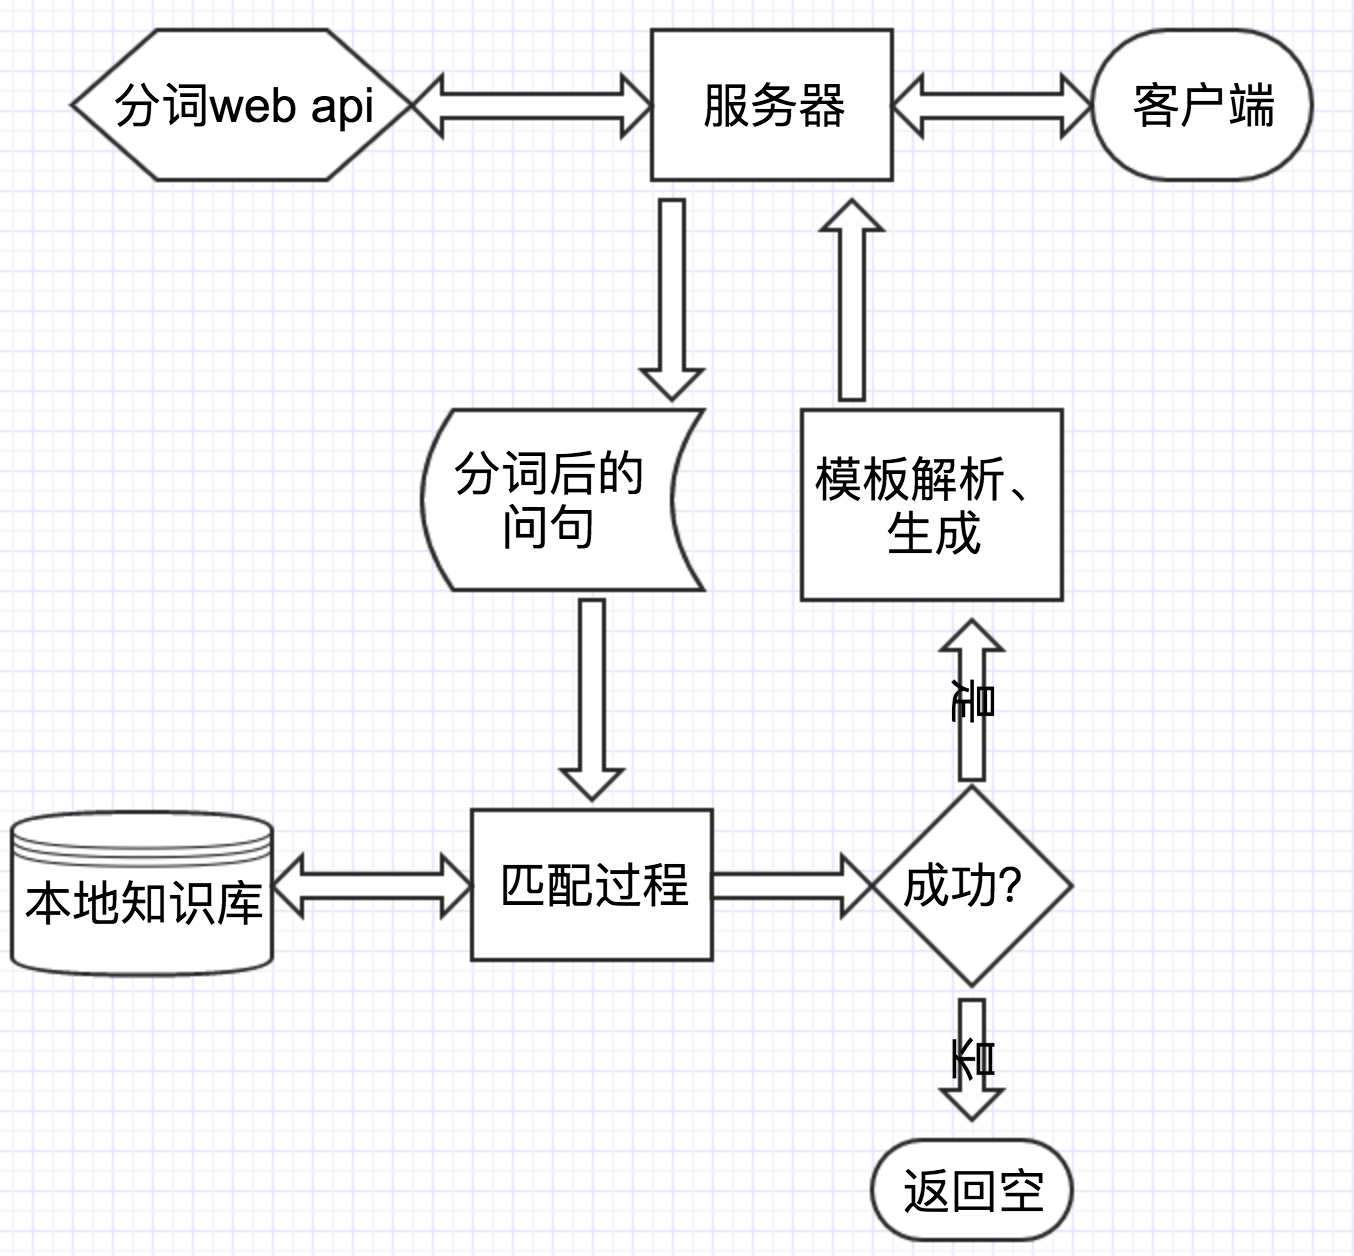
\includegraphics[width= 0.8\textwidth]{flow-chart.png}\\
  \caption{系统的结构和工作流程}\label{fig:pic3}
\end{figure}


下面介绍代码构成。在图\ref{fig:pic4}中 A 部分所指的是前端代码,前端使用 AngularJS 框架,项目结构严格按照 AngularJS guide 的要求构建,采用 MVC 的结构,组件化开发。项目使用 webpack 打包,webpack.config.js 文件是作为本地开发时候的测试构建的配置文件,而 webpack.prod.config.js 是最后部署的时候使用的配置文件。webpack 的作用是,使得 javascript, html, css, scss 文件都能通过 ES6/CommonJS 的 import/require 语句来导入,且不用担心最终打包的内容中各个文件的路径解析的问题,这使得开发环境的目录可以按照不受最终浏览器请求的目录的限制。下面看代码文件,主窗口是 ChatWindow,这是最上层的容器,然后该容器内有三个组件(components文件夹下),chattingContainer 是聊天时候的内容容器,也就是用户聊天记录显示的地方,该容器支持动态滚动,既会随着新消息的到来自动滚动;inputContainer 是聊天时候的输入容器,该部分包括一个输入框和一个发送按钮;sidebarContainer 是左侧的登录注册页面,支持自动弹出,以及点击空白自动缩回。其他的就如文件夹的名字所示,是静态资源。

在图\ref{fig:pic4}中 B 部分所指的是聊天机器人(Json Robot)代码。aiml\_corpus 文件夹里的是 AIML 格式的语料库,可以通过 utils/aiml2json.py 来将其转换成 Json Robot 自己的语料库。转换后的内容会被放到 trainning\_data 文件夹下面。该文件夹下的文件,在启动训练的时候,会全部被转换到 running\_data 目录下,成为最终的“大脑”存放的结果。Json Robot 的核心在 Core 文件夹下面,在 brain.py 文件中包含了聊天机器人所有的功能,初始化,训练,搜索,更新,销毁。在 parse.py 中提供了一些公共的解析函数。server 文件夹下面是 flask app 注册的地方。utils 文件夹下面有,第三方 api 调用的接口函数,以及各种参数的设置。tests 文件夹下面是单元测试,用的 pytest 工具。系统源码结构请看图\ref{fig:pic4}。

\begin{figure}[htbp]
  \centering
  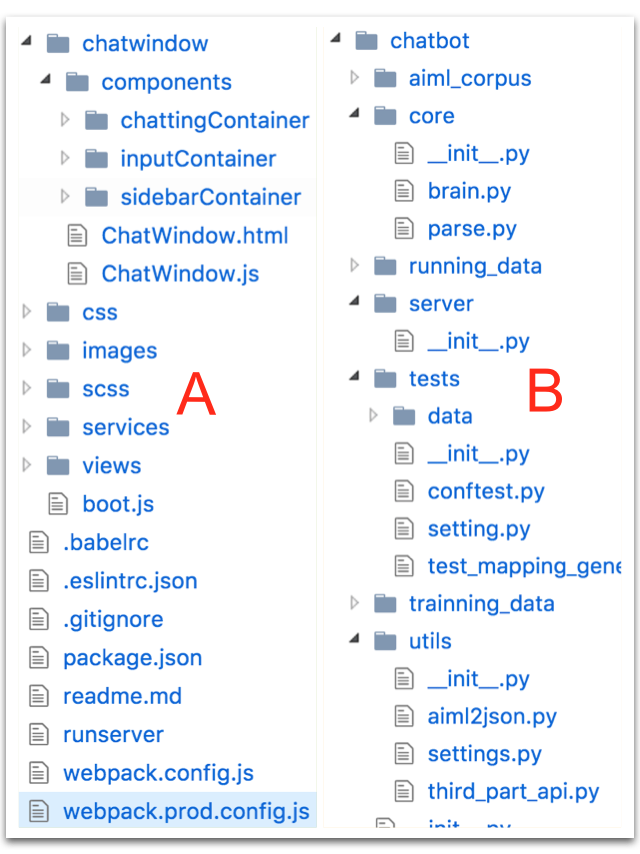
\includegraphics[width= 0.5\textwidth]{source-code.png}\\
  \caption{系统源码结构图}\label{fig:pic4}
\end{figure}



\section{聊天机器人}
\subsection{json文件解析和处理}

Json Robot 的创新之处就在于它摒弃了 AIML 的语法,自己设计了一套基于 JSON 的模板书写规则。下面就看看这套新的语法是怎么样的。下面的例子是单个文件的 json 模板。

\begin{lstlisting}[language=]
[
    {
        "ask":  ["你好S","你好", "U你好S", "U你好"],
        "reply": ["你好。"]
    },
    {
        "ask": ["S"],
        "reply":[
            "呀,这个问题我不会。",
            "您能换一种问法吗?",
            "呀,我听不懂。"
        ]
    },
    {
        "ask":  ["U搜S","搜S","知道S", "你知道S", "U是什么", "U是什么S"],
        "reply": ["T{百度}"]
    }
]
\end{lstlisting}

在这个 json 文件中,我们可以看到,最外层是一个数组,这个数组的元素是一些字典。正如之前所说的 AIML 最小的记忆单元是 <category> ,Json Robot 知识库的最小记忆单元就是这些字典了。字典里的内容非常简单,只有"ask"和"reply" 两个键值对,顾名思义,前者是问句,后者是回答,对比 AIML 中的 <pattern> 和 <template> 。然后在问句中我们看到 "S" 和 "U" ,它们代表的意义就是原来的 "*" 和 "\_" (Star 和 Underscore)。这些字母提供了类似于正则表达式的功能,具体请看AIML Match Pattern \cite{aiml-match-pattern}。然后,在第一个字典中,我们可以看到,多个问句(ask 的值为一个数组)对应了一个回答,这一设计解决了 AIML 书写冗余问题。然后第二个字典中,一个问句(此处是根节点,既所有匹配不到结果的问题最终都会返回此处的内容),对应了对个回答(reply 的值是一个数组),这些回答将会在程序中随机返回给用户。在第三个字典中,我们看到最后的回答内容是 T 开头的,这表示此处的内容需要交给模板处理函数来处理,模板处理函数会提取这里的关键词(百度),然后根据关键词去执行操作,最后返回特定的内容,此处将返回百度百科搜索到的内容。

另外,程序还提供了一个 AIML 到 JSON 文件的转换功能。可以很方便的把社区维护的 AIML 语料库集成到此聊天机器人身上。

\subsection{核心模块功能}

从程序的最高层,也就是向外暴露的 API 开始分析。Core 类拥有四个方法,ask,trainning,rebuild,run。先看程序是如何训练这些 JSON 文件到本地文件系统中去的。

\begin{lstlisting}[language=Python]
    def saving_and_update_brain(self, input_dict):
        for asking_str in input_dict['ask']:
            generated_dir = os.path.join(self.running_data_dir,
                                         '/'.join(pattern_list))
            generated_full_path = os.path.join(generated_dir, 'template.json')

            template_json = input_dict['reply']
            # save file
            if not os.path.exists(generated_dir):
                os.makedirs(generated_dir)
            with open(generated_full_path, 'w+', encoding='utf8') as fp:
                fp.write(json.dumps(template_json, ensure_ascii=False))
            self.update_brain(pattern_list)
\end{lstlisting}

这部分代码为了消除噪音,我做了删减。实际上上面代码做的事情是,把输入”你好吗S“进行分词,结果为”["你","好","吗","S"]“,然后将这个数组合并后作为这个模板的路径,既最后的回答会在,/你/好/吗/\%S/template.json 文件里面。然后 update\_brain 函数会再更新索引文件(index.json)。


然后进入 ask 方法,看看当我们询问一句话的时候,程序会怎么查找。

\begin{lstlisting}[language=Python]
 def _search(self, words, root):
        # for 'U(nderscore)'
        if len(words) == 0:
            return root['word'] if root.get('isLeaf') else None

        index = self._get_index_in_nodes_list("%U", root)
        if index != -1:
            next_node = root['child_nodes'][index]
            for i in range(len(words)):
                suffix = words[i + 1:]
                mid_result = self._search(suffix, next_node)
                if mid_result:
                    return root['word'] + '/' + mid_result
\end{lstlisting}

这部分代码同样做了删减。此处算法就是之前提到的 AIML Match Pattern 论文\cite{aiml-match-pattern}里的实现。正在处理的是 "\_" 这个字符,将所有长度的子串去递归查找一次。终止条件是找到了叶子节点。

\subsection{单元测试}

好的测试,是保证程序稳定运行的关键。不一定要遵循 TDD 的策略来开发,但是得及时将测试补上。本项目每增加一个新的功能,都会增加新的测试。

基本的查找测试。

\begin{lstlisting}[language=Python]
def test_searching():
    assert '/%U/天空/是/什么/颜色/%S' == brain.search_brain('你知道天空是什么颜色吗?')
    assert '/%U/再见' == brain.search_brain('那再见')
    assert '/%U/再见/%S' == brain.search_brain('那就再见吧!')
    assert '/再见' == brain.search_brain('再见')
\end{lstlisting}

第三方 API 调用的 mock 测试。

\begin{lstlisting}[language=Python]
def test_reply_template_generate():
    @urlmatch(netloc=r'(.*\.)?baike\.baidu\.com$', path=r'.*')
    def baidu_mock(url, request):
        return ''
    with HTTMock(baidu_mock):
        assert "你是说 圆周率 吗?不知道QAQ" == \
            brain.open_template(brain.search_brain('你知道圆周率是多少吗'))
        assert "你是说 圆周率 吗?不知道QAQ" == \
            brain.open_template(brain.search_brain('帮我搜一下圆周率'))
\end{lstlisting}

\section{用户界面}

主界面的外观模仿我们通常使用的聊天软件。既具备对话框,输入框,发送按钮,菜单等基本功能。

\subsection{需求描述}
本论文设计了一个通用的聊天机器人开发规则,精华聚集在了后端聊天机器人的内容上,因此用户界面部分要以突出聊天机器人能回复的内容为核心来展现。由此可以提出基本的需求如下。
\begin{enumerate}
\item 聊天窗口。具备自动滚动功能;用户发送的和机器回复的内容有明显的区分;随着屏幕大小的调整自动适应。
\item 输入框。具备文字输入功能,用户可以通过回车或者点击右侧的发送按钮来发送内容。
\end{enumerate}

另外,可以随着业务规模的增大,添加其他的功能,比如用户注册,后台管理,自定义训练内容等等。


\subsection{设计思路和效果图}

界面采取 Material design 的深色风格,主界面的核心伪代码如下。

\begin{lstlisting}[language=C]
export default angular.module('chatWindow', ['ngMaterial', 'luegg.directives'])
.controller('chatwindowCtrl', ['$scope', '$timeout', 'jsonbotService', function($scope, $timeout, jsonbotService) {
    ...
}])
.component(sidenavContainer.name, sidenavContainer.config)
.component(chatWindow.name, chatWindow.config)
.component(chattingContainer.name, chattingContainer.config)
.component(inputContainer.name, inputContainer.config)
.service('jsonbotService', jsonbotService);
\end{lstlisting}

从这里可以看到,组件化开发的好处,sidenavContainer, inputContainer, jsonbotService 顾名思义分别是左边栏窗口组件,输入框组件,聊天机器人的服务组件。这样解耦开来的代码可以让项目随时往上迭代。

主界面和用户聊天的实时截图。

\begin{figure}[H]
  \centering
  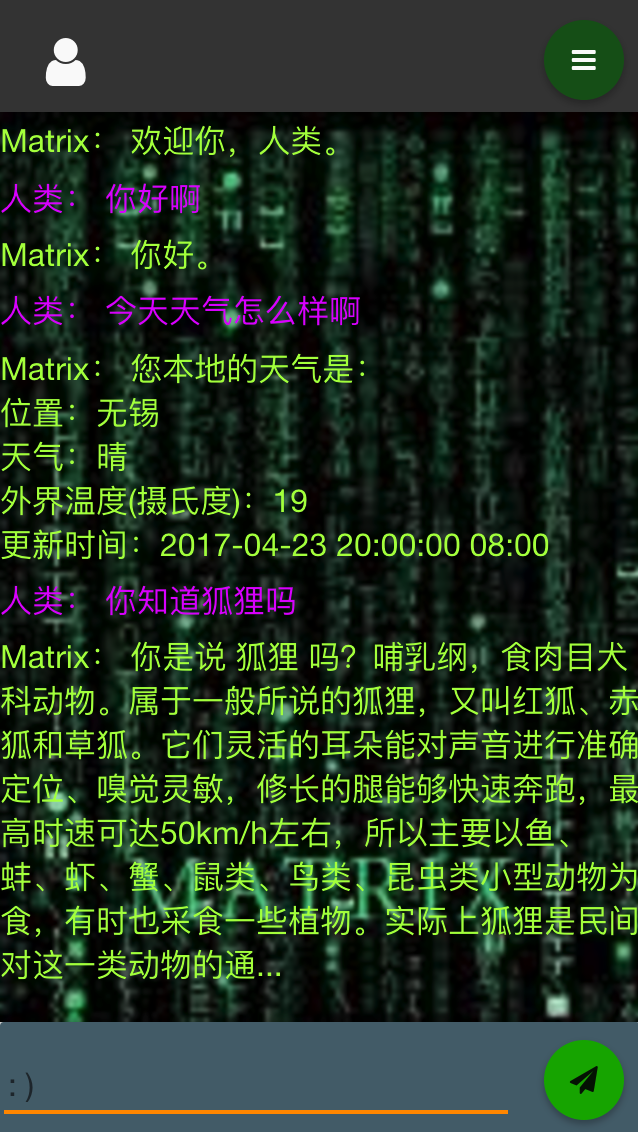
\includegraphics[width= 0.5\textwidth]{chat4.png}\\
  \caption{用户聊天截图}\label{fig:pic6}
\end{figure}

从图\ref{fig:pic6}中可以看到,可以向聊天机器人询问天气,这里返回的是当地的实时天气,包括位置,气象和温度三个参数。它背后调用的第三方专门的天气接口,数据返回速度取决于当时的网络情况。当询问的语句是,你知道* ,或者 帮我搜* ,这种格式的时候,首先会提取句子里的关键词,这里是“狐狸”,然后会自动搜索百度百科的内容,如上所示结果返回了关于狐狸的词条。

\begin{figure}[H]
  \centering
  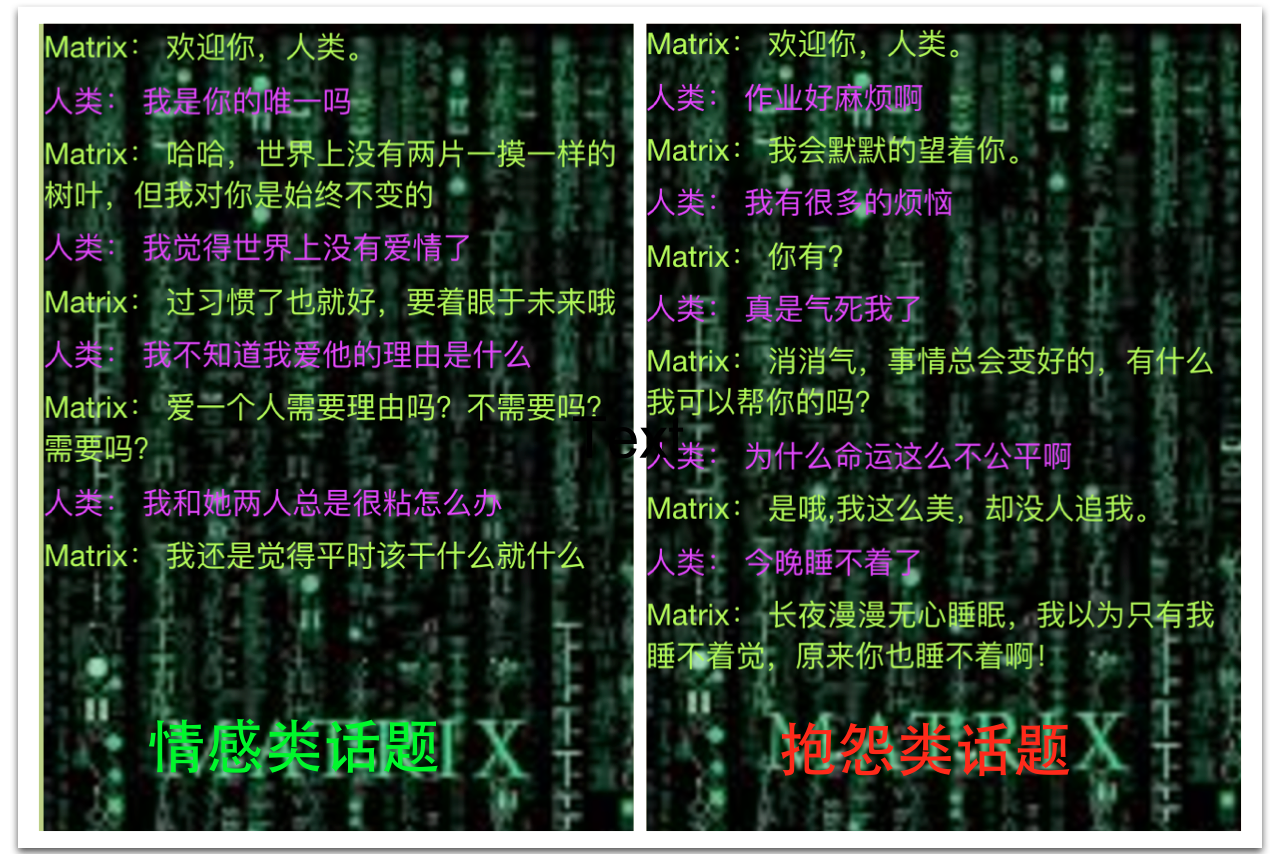
\includegraphics[width= 1.0\textwidth]{chattopic.png}\\
  \caption{不同聊天话题截图}\label{fig:pic7}
\end{figure}

从图\ref{fig:pic7}可以看到聊天机器人能回答情感类的和抱怨类的话题,其实整个知识库总共支持二十多种类型的回复主题,这些主题都是从之前的 AIML 积累的知识库转换而来的,具体有哪些主题请看表\ref{table:t3}。

\begin{table}[H]
  \centering
  \begin{tabular}{p{38mm}p{38mm}p{38mm}}
    \toprule
    \textbf{话题} & \textbf{话题} & \textbf{话题}\\
    \midrule
    Greeting, Complain, Discuss, Encourage, External, Film, Food, Game & Healthy, Inherence, Internet, Job, Joke, Life, Music & Master, Plan, Rude, Sentiment, Sex, SmallWord, Travel, gossip\\
    \bottomrule
  \end{tabular}
  \caption{JsonBot 支持的聊天话题}\label{table:t3}
\end{table}


用户登录页面,采取左侧弹出的形式。此论文里没有实现的必要,故只实现了 UI ,没有实现真正的后台。下面是实现代码和截图。

\begin{lstlisting}[language=C]
export default {
	name: 'sidebarContainer', 
	config: {
		controller: ['$scope', '$mdSidenav', function($scope, $mdSidenav){
            ...
		}],
		bindings: {issidebarToggle:'='},
		template: sbhtml
\end{lstlisting}


\begin{figure}[H]
  \centering
  
\includegraphics[width= 0.5\textwidth]{chat2.png}\\
  \caption{用户登录页截图}\label{fig:pic8}
\end{figure}


训练按钮。因为目前的语料库构建好之后,被用户私自改动是很难再改回来的,所以目前没有支持该功能的打算,只是提供展示。下面是实现代码和截图。

\begin{lstlisting}[language=C]
export default {
	name: 'inputContainer', 
	config: {
		controller: ['$scope', function($scope){
			...
			};
		}],
		bindings: {
			inputedCallback:'&'
		},
		template: iphtml
	}};
\end{lstlisting}

\begin{figure}[H]
  \centering
  
\includegraphics[width= 0.5\textwidth]{chat3.png}\\
  \caption{训练按钮截图}\label{fig:pic9}
\end{figure}




\chapter{总结与展望}
\section{论文总结}

聊天机器人在如今是热点,无论是客服聊天还是私人助理,聊天机器人都能给我们的生活带来便利,减轻人类的工作压力,减少重复劳动的乏闷。

本文在分析了 ALICE 的工作原理的情况下,深度剖析了它的优缺点。提出并实现了一个全新版本的聊天机器人。并且取其精华,去其糟粕,使得本论文实现的聊天机器人拥有同样的功能,却需要更低的学习成本和开发成本。论文的具体工作如下。

\begin{enumerate}
\item 搜集了大量资料、文献。追根溯源,了解了聊天机器人的发展历史,以及截止到目前的国内外发展水平。以此保证论文的观点与时俱进。
\item 分析了经典的聊天机器人模型 ALICE ,一步一步根据数据流向,追踪并且分析了Python 版本的 ALICE 源代码。然后分析了 ALICE 的“大脑” AIML 文件。介绍了它的标签集合,并分析了部分内容。
\item 介绍了常见的分词算法,和本文用到的分词服务。
\item 选择 Python 语言设计了一个比 ALICE 更容易使用和开发的聊天机器人。同时设计了新的“大脑”文件的书写规范,使得用户不再需要预先学习大量的标签库了。
\item 使用 AngularJS 开发了一个用于演示的web app界面,来展示这个聊天机器人。
\end{enumerate}

然而,本论文还有很多不足。对目前的实现来说,构建好的知识库没有一个良好的热更新策略,而且也没有修改的策略,那些坏数据,会永远保留在文件树内。目前的做法是删除整个知识库,然后重新构建。这种方法在知识库少的时候很有效,但当知识库庞大起来,删除和重建所消耗的时间资源很难想象。

\section{不足和展望}

用户界面设计不够人性化,交互体验差,用户使用兴趣低。可以专门设计一下 UI。

Web 界面只支持移动端,可以增加 PC 端实现。

程序的日志输出和异常处理做的还不够,未到达产品级别的要求。未来可以增加日志输出,接入日志管理系统例如 Sentry 等。

程序接口的文档不足,会给开发者带来困难。未来可以补上文档。

由于目前的分词工具用的是第三方 web api 服务,而分词的需求又非常频繁,而请求时间又依赖于与网络情况,因此采取本地分词会是一个更好的决策。目前可以想到的方法有,直接用结巴分词的 Python 实现;也可以用自己的 Python 代码去调用结巴分词的C++库。

知识库的构建不够。由于此类聊天机器人都是依赖于人工编写的知识库,因此很难达到理想情况下的“足够”。只能一点一点依靠社区积累。

% 参考文献
\nocite{*}
\bibliography{bachelor}

\begin{acknowledgement}
  本论文在我的导师徐华老师的悉心指导和作者的努力之下,终于圆满完成了,感谢我的指导老师对我论文的帮助,感谢朋友,以及开源社区的贡献者们,对我项目开发和实现过程中的指导。你们的耐心和无私,让我在开发和设计过程中,少走了很多弯路。我深深的感受到了自己在本科阶段的进步,以后在工作上一定也会保持独立思考的习惯,勤奋工作,期待达到更高的层级。现在我可以骄傲地给我的本科阶段画上一个完美的句号了。细细地回顾这段时光,内心里的感激之情溢于言表。

  其次,我还要感谢我的班主任,蒋敏老师。从刚入学教我们离散数学开始,我就被蒋老师的严谨缜密的讲课风格所深深吸引。在后面的几年里,蒋老师给了我很多发展的机会,包括做项目和去学校外面实习。这些珍贵的锻炼机会对我的影响很大,我目前能得到的一切都离不开老师的敦敦教诲和提拔。

  同时我还要感谢我的室友,社团的学长们。正是我们之间的技术讨论,交流还有竞争,让我明白了人生如逆水行舟,不进则退。当你还在迷茫的时候,别人已经翻过了好几座山峰了。感谢你们的陪伴,感谢所有的朋友们。

  再次,感谢我的父母,一直陪伴着我的求学生涯,给了我最好的条件,今天的我有一半的功劳归功于他们,离不开他们的无私奉献,离不开他们的爱。

  最后,向所有百忙之中审阅本论文和参与答辩的所有老师致以由衷的感谢,谢谢你们给我提出的意见和建议,我会始终保持虚心的态度,向您们学习。

\end{acknowledgement}
%%%%%%%%%%%%%%%%%%%%%%%%%%%%%%%%%%%%%%%%%%%%%%%%%%%%%%%%%%%%%%%%%%%%%%%%%%%%%%%
\end{document}